\presec \section{Asymptotic Form of the FP Probability} \postsec \label{sec:limitf}
%
In this section, we derive a new approach to computing the asymptotic form for the FP probability of BFs. 
%
The new derivation is based on \textit{partitioned Bloom Filters} (pBF) that are used frequently to carry out parallel queries. 
%
Its underpinning principle is simple: the BF is divided into $k$ even partitions, and each hash function only acts on one of the partitions, respectively.
%
The probability that one bit of the BF array remains 0 after inserting $n$ elements in the BF becomes the following as now each hash maps into $\frac{m}{k}$ separate bits.
%
\begin{equation}
p'_{partition} = \left( 1-\dfrac{k}{m} \right)^n
\label{equ:p'pBF}
\end{equation}

It is intuitive that the FP probability of partitioned BF is a little bigger than that of BF. 
%
Unfortunately, there is no strict proof. 
%
Here we show one proof method, which is based on the following Lemma. 

\vspace{0.05in}
\noindent\textbf{Lemma II:} For $m > 1 \;\;,   k >1, \;\; n > 1, \: m>k$,
\begin{equation}
\label{theorem1}
\left( 1-\dfrac{k}{m} \right)  ^n <
\left( 1-\dfrac{1}{m} \right)  ^{kn}
\end{equation}

\begin{proof}
Note that when $m$ is large, the left expression approximates to the right one. Below we give the derivation details.
%
Let $g(k)=( 1-\frac{1}{m} )  ^k- ( 1-\frac{k}{m} )$. 
%
For $m>1$ and $k>1$, $g(k)$ is a continuous and derivable function, and we can obtain the following inequality in terms of its derivative:
%
\begin{equation}
\begin{aligned}
%g'(k)=k\left( 1- \dfrac{1}{m}\right) ^{k-1} +\dfrac{1}{m}
g'(k) %&=\left( 1- \dfrac{1}{m}\right)^k \ln\left(1-\dfrac{1}{m}\right)+\dfrac{1}{m} \\
> \left( 1- \dfrac{1}{m}\right)\ln\left(1-\dfrac{1}{m}\right)+\dfrac{1}{m}
\end{aligned}
\end{equation}
%
Let $f(m)=\left( 1- \dfrac{1}{m}\right)\ln\left(1-\dfrac{1}{m}\right)+\dfrac{1}{m}$.
%
Then $f'(m) = \dfrac{1}{m^2} \ln\left(1-\dfrac{1}{m}\right)< 0$, which means that the function $f(m)$ is strictly decreasing.
%
When $m$ goes to infinity, we have $\lim\limits_{m \to \infty}  f(m) =  0$. 
%
Therefore, we know that $f(m) \geqslant 0$, and $g'(k) > f(m) \geqslant 0$, which means that the function $g(k)$ is strictly increasing.
%
Thus, we have
%

\begin{equation}
\left( 1-\dfrac{k}{m} \right) ^n   <
\left( 1-\dfrac{1}{m} \right)  ^{kn}
\end{equation}
\end{proof}

The above lemma shows that $p'_{partition} < p'_{true}$ or equivalently $1-p'_{partition} > 1-p'_{true}$.
%
Thus, we know that with the same parameters, the FP probability of the pBF will be larger than that of the standard BF $f_{true}$, \ie, $f_{partition} > f_{true}$. 
%
In addition, Bose’s bounds in Eq. \ref{fBound} state that the precise value of FP probability for a BF $f_{true}$ is larger than $f_{bloom}$, \ie, $f_{true} > f_{bloom}$. 
%
Therefore, we have the following upper and lower bounds:

\begin{equation}
\label{bigbig}
f_{partition} > f_{true} > f_{bloom}
\end{equation}

For a partitioned BF, the probability that one bit of the array is still 0 $p'$ is shown in Eq. \ref{equ:p'pBF}.
%
Different from standard Bloom Filters, for a partitioned Bloom Filter, the event $E(h_1=1),E(h_2=1),E(h_3=1),...,E(h_{i-1}=1)$ is independent of the event $E(h_{i-1}=1)$, where $E(h_{i-1}=1)$ means that the event that the position of $h_{i-1}(x)$ is 1 because each hash function is responsible for one partition, and has no impact on each other. 
%
Therefore, we have
%
\begin{equation}
f_{partition}=(1-p'_{partition})^k=\left( 1- \left( 1-\dfrac{k}{m} \right)^n \right) ^k
\end{equation}
Then the formula~\ref{bigbig} becomes

\begin{equation}
\label{bounds}
\left( 1- \left( 1-\dfrac{k}{m} \right)^n \right) ^k > f_{true} > \left( 1- \left( 1-\dfrac{1}{m} \right)^{nk} \right) ^k
\end{equation}

Then we use the well known limit formula:
\begin{equation}
\lim\limits_{x \to \infty} \left( 1-\dfrac{1}{x}\right) ^{-x} = e
\end{equation}

%%
Asymptotically, when $m$ becomes large, we already know that $f_{bloom}$ converges to the term in Eq. \ref{fBloom}. 
%
Nevertheless, the upper bound has also an asymptotic behaviour as the following, which is the same term as the lower bound limit. 
%
\begin{equation}
\label{flim}
\lim\limits_{m \to \infty} \left(1-\left(1-\frac{1}{m}\right)^{nk}\right)^k = \left(1-e^{-nk/m}\right)^k 
\end{equation}
%
Through the Sandwich Theorem (also known as squeeze theorem) we obtain the following equation, which is similarly to Christensen and Bose:
\begin{equation}
\label{flimtrue}
\lim\limits_{m \to \infty}  f_{true} =  \left(1-e^{-nk/m}\right)^k 
\end{equation}

This means that when $m$ is large, the Bloom's formula can be used with negligible error. 
%
However, we still need to evaluate what means \textit{$m$ being large}. 
%
We will do this by comparing the two bounds we have in hand: the one from Bose and the one we derived in this paper.
%
We show in Figure~\ref{fig:uplowbound} that the two upper bounds along with the lower bound obtained for $k=7$  and $m=10n$ as a function of $n$, the number of elements inserted in the BF.
%
As can be seen, the upper bound derived in this paper and the lower bound $f_{bloom}$ converge relatively fast for $n=9$, while the upper bound derived by Bose has a much slower convergence. 
%
We can see this better by looking at the behavior of the bounds error ratio $\beta$, defined as $\beta=\frac{upper\ bound - lower\ bound}{lower\ bound}$, for the two bounds in Figure \ref{fig:ratio}.

\begin{figure}[t]
\centering
\prefig
\vspace{-0.1in}
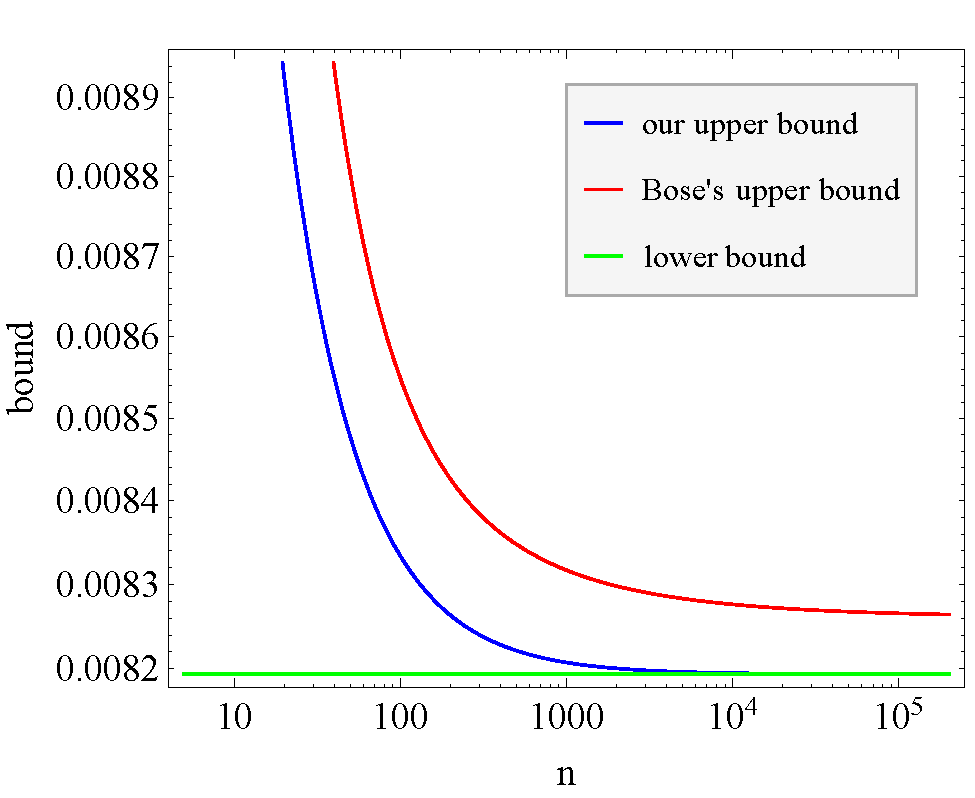
\includegraphics[width=\figwidth]{LogLog_lowerUpper}
\postfig\precaption
\vspace{0.1in}
\caption{Upper and lower bound for $f_{true}$ for $k=7$ and $m=10n$.} 
\postcaption
\vspace{0.1in}
\label{fig:uplowbound}
\end{figure}

\begin{figure}[t]
\centering
\prefig
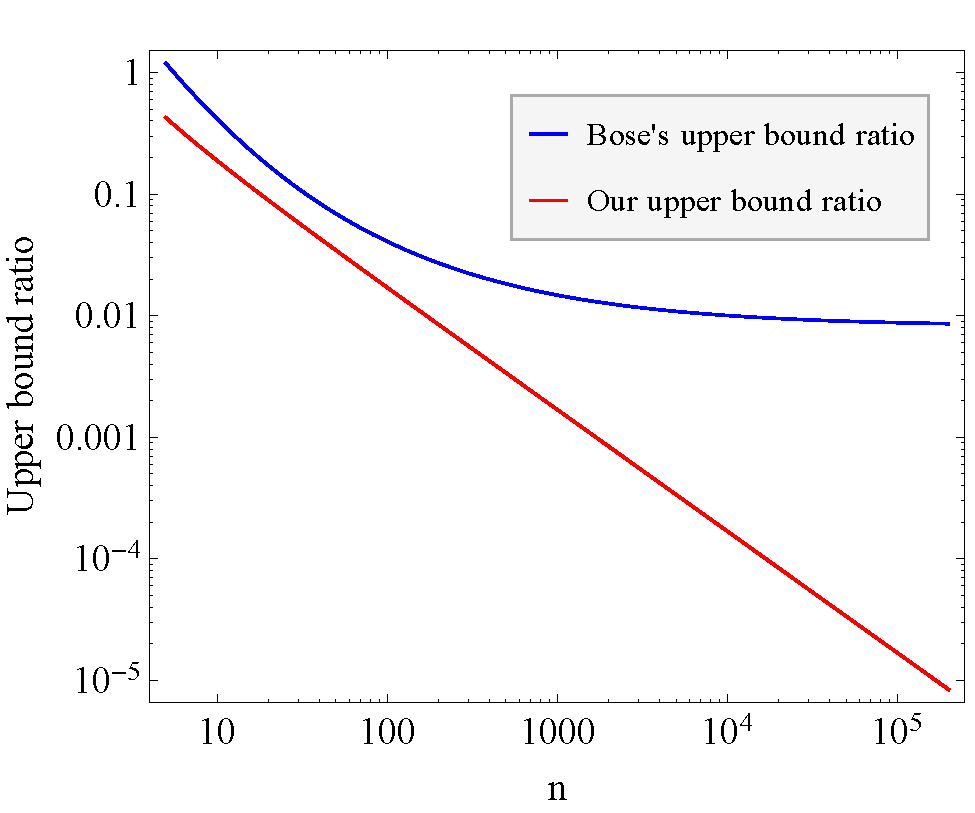
\includegraphics[width=\figwidth]{LogLog_ratio}
\postfig\precaption\vspace{0.1in}
\caption{Bounds error ratio for Bose's bound and the bound derived in this paper for $k=7$ and $m=10n$. } 
\postcaption
\vspace{0.1in}
\label{fig:ratio}
\end{figure}

As can be seen, the gap between our derived upper bound and $f_{bloom}$ is decreasing polynomially at a constant speed, while Bose's bound has a lower speed of convergence. In order to extend this observation, we show in Figure \ref{fig:ratiok} the evolution of the bounds error ratio for a BF with $m=10000$, $n=1000$ and varying $k$. 

\begin{figure}[htbp]
\centering
\prefig
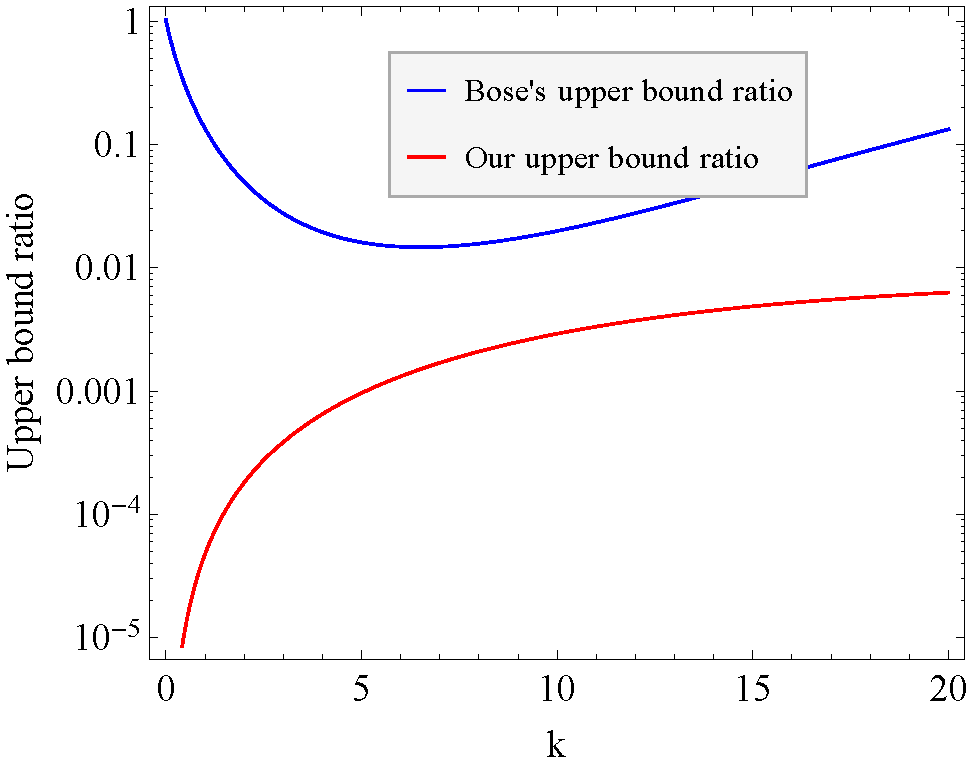
\includegraphics[width=\figwidth]{ratioLog_k}
\postfig\precaption\vspace{0.10in}
\caption{Bounds error ratio for Bose's bound and the bound derived in this paper for $m=10000$, $n=1000$ and varying $k$.}  
\postcaption
\vspace{0.1in}
\label{fig:ratiok}
\end{figure}

As expected, error involved with using $f_{bloom}$ increases with the number of hash functions $k$ increases. 
%
However, it can be seen that the convergence behavior of the bounds derived in this paper is much better than the one obtained by Bose. 

\begin{comment}
The calculation of the correct rate of the counting Bloom filter \cite{cbf}, $\mathcal{C}_r$, can benefit from our derivation about the false positive probability of standard Bloom filter. 
%
The counting Bloom filter (CBF), one variant of standard Bloom filter, replaces each bit with one counter, supporting estimating the frequency of each inserted item. 
%
In CBF, the over-estimation of an inserted item is equivalent to one false positive in standard Bloom filter. 
%
Therefore, we have: 
\begin{equation}
\mathcal{C}_r = 1 - f_{true}
\end{equation}
%
Applying equation \ref{bounds}, we can get the upper and lower bounds of the $\mathcal{C}_r$ of CBF. 
\end{comment}
